\section{Preliminaries}
Consider a robot equipped with sensors navigating an environment toward a designated global goal $g_{\textrm{global}} \in \mathbb{R}^2$. This task can be broken into a sequence of local navigation subtasks, where the robot moves toward intermediate local request goals $\mathcal{G}_{\textrm{local}}$, determined by a global planner based on the nearby segmented terrain polygons $\mathcal{P}$. We illustrate an instance of such a local task setup.
% following the same example introduced in \citep{zhou2025physically}.
% throughout the paper.

\noindent
\textbf{Example~\examplelabel{example:1}}.
% (9-grid locomotion). 
\textit{
Consider a 2D grid world with nine cells (in yellow) in Fig.~\ref{fig:preliminary_nine_squares}. The robot is required to move from an initial cell (e.g. the center cell) 
to a desired goal cell indicated by the star. 
Each cell is assigned a terrain type, such as $\textit{Dense}$ or $\textit{Sparse}$ stepping stones.}

%%%%% Fig. 9 grid %%%%
\begin{figure}[ht]
    \centering
    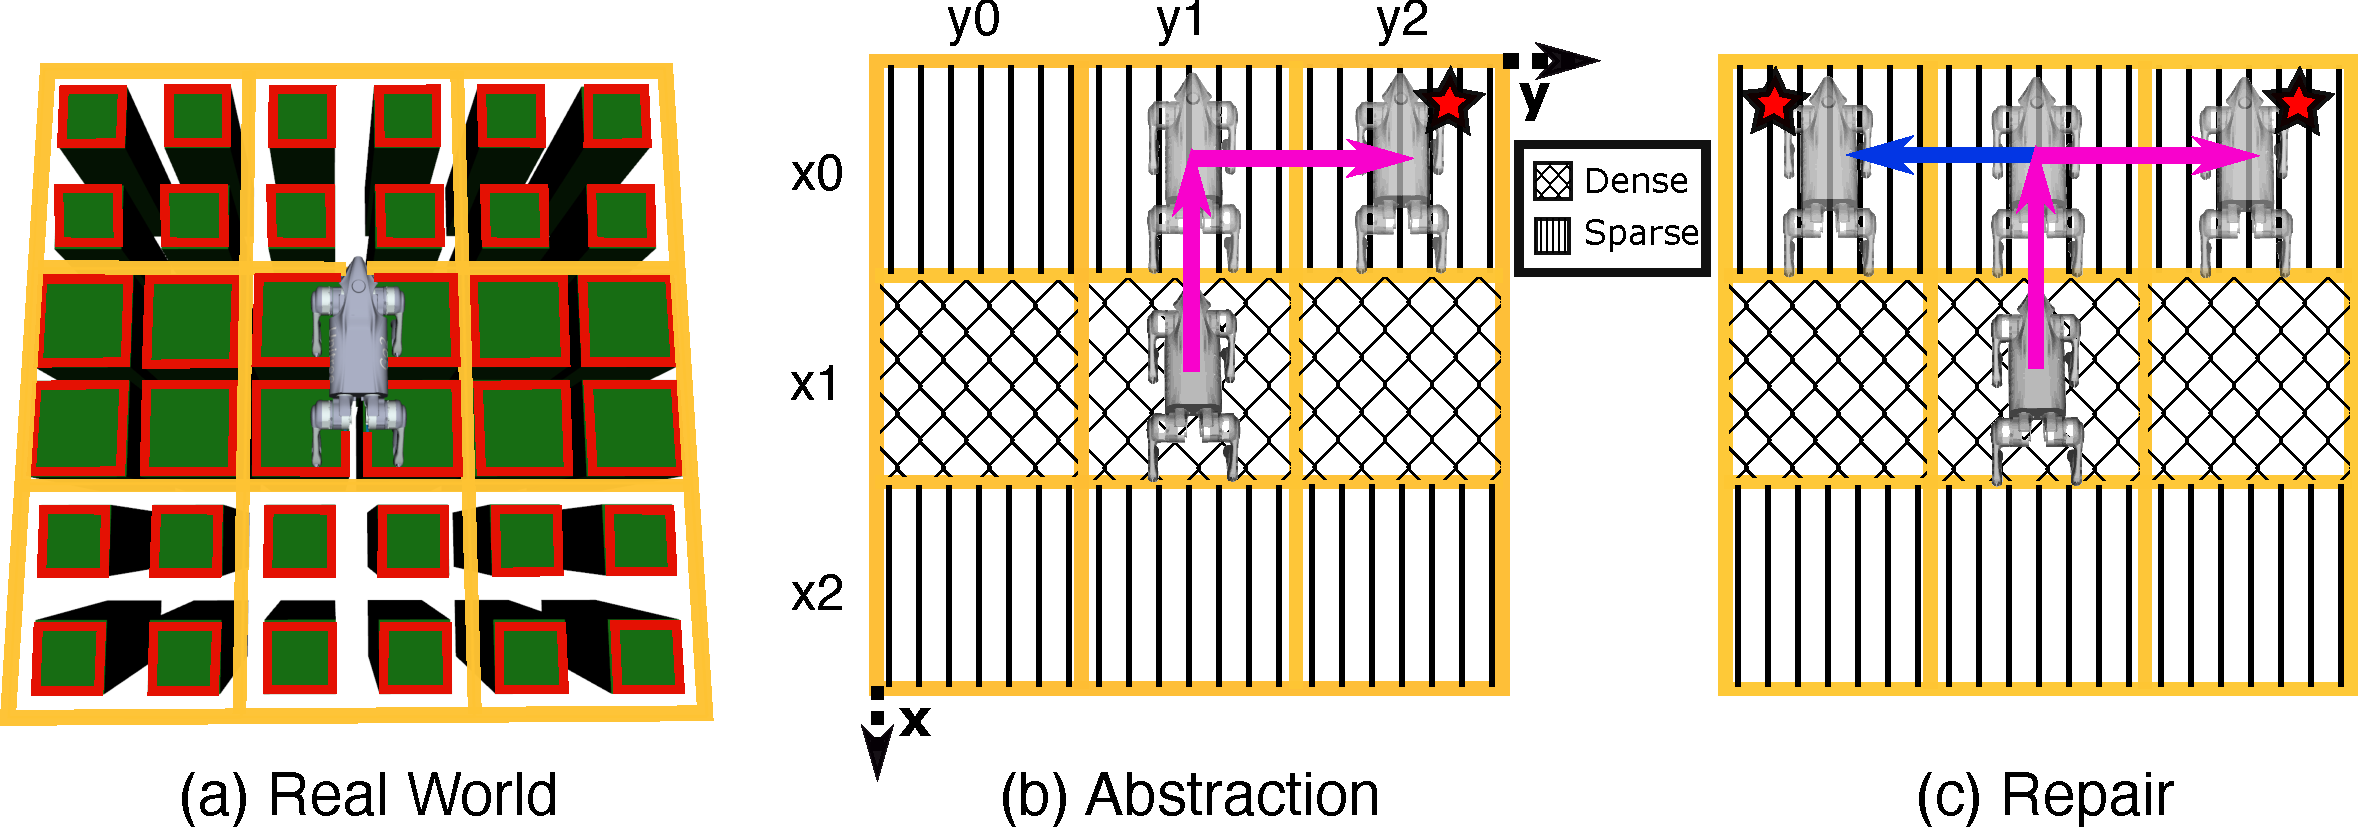
\includegraphics[width=\linewidth]{preliminary_drawing.pdf}
    \caption{Terrain abstraction and skill definition. (a) Top-down view of the real-world terrain before abstraction. The red polygons denote the segmented terrain polygons. (b) Abstraction of the terrain and robot's skills (pink) moving from one location to another. (c) Repair process to find a new skill (blue).}
    \label{fig:preliminary_nine_squares}
\end{figure}
%%%%%%%%%%%%%%%

\subsection{Abstractions}\label{sec:preliminaries_abstraction}

% Given a set of terrain polygons $\mathcal{P}$,
% e.g.,
% in Fig.~\ref{fig:preliminary_nine_squares}(a),
% we abstract them into a 2D grid of size $n\times m$.
% For each dimension,
% we denote each location in that dimension with a symbol,
% resulting in two sets
% $\xcells \coloneqq \{x_0, \dots, x_{n-1}\}$
% and
% $\ycells \coloneqq \{y_0, \dots, y_{m-1}\}$.
% %
% We define a set of atomic propositions 
% $\ap$,
% partitioned
% into sets of inputs $\mathcal{I}$
% and outputs $\mathcal{O}$,
% to describe the symbolic world states and robot actions.
% The inputs $\mathcal{I}$ consist of
% the robot inputs 
% $\inpcen$,
% the request inputs 
% $\inprequest$,
% and
% the terrain inputs $\inpterrain$
% ($\inp = \inpcen \cup \inprequest \cup \inpterrain$).
% The robot inputs 
% $\inpcen \coloneqq 
% \{\var_x \mid x \in \xcells\} \cup 
% \{\var_y \mid y \in \ycells\}$
% are used to abstract the robot position,
% the request inputs
% $\inprequest \coloneqq
% \{\var_x^\textrm{req} \mid x \in \xcells\} \cup 
% \{\var_y^\textrm{req} \mid y \in \ycells\}
% $
% are used to abstract the requested goal cells,
% and
% the terrain inputs
% $\inpterrain \coloneqq \{
% \tvar{x}{y} \mid x\in \xcells, y\in \ycells
% \}$
% describe 
% the terrain type of the grid cells.
% %
% The robot state can be extended to incorporate orientation information, such as the floating base's yaw angle, as demonstrated in Sec.~\ref{sec:extension}.
% We then consider a finite set of size $n_t$ of terrain types, 
% defined based on their physical characteristics. 
% For $\physicalstate \in \naturals$, we denote $\range{\physicalstate} \coloneqq \{0, \dots, \physicalstate - 1\}$.
% We note that 
% terrain inputs $\tvar{x}{y} \in \inpterrain$
% are integer variables
% belonging to $\range{n_t}$,
% and we translate them into a set of Boolean propositions,
% as done in~\citep{ehlers2016slugs}.
% %
% An input state 
% $\inpstate$
% is 
% a value assignment function
% $\inpstate: \inp \to \{\true, \false\} \cup \range{n_t}$. Since the robot can only be in one cell at a time, and the goal is a single cell, we require that exactly one $\var_x$, one $\var_y$, one $\var_x^\textrm{req}$, and one $\var_y^\textrm{req}$ be $\true$, for each input state. 
% The robot states $\inpstatecen: \inpcen \to \{\true, \false\}$,
% request states
% $\inpstaterequest: \inprequest \to \{\true, \false\}$,
% and
% terrain states
% $\inpstateterrain: \inpterrain \to \range{n_t}$
% are the projections of $\inpstate$ on 
% $\inpcen$,
% $\inprequest$,
% and $\inpterrain$, respectively.
% We denote the sets of input states as $\inpstates$,
% robot states as $\inpstatescen$,
% request states as $\inpstatesrequest$,
% and 
% terrain states as $\inpstatesterrain$.

Given a set of terrain polygons $\mathcal{P}$, such as those in Fig.~\ref{fig:preliminary_nine_squares}(a), we abstract them into a 2D grid of dimension $n \times m$. For each axis, we label every position with a symbol, producing two sets: $\xcells \coloneqq \{x_0, \dots, x_{n-1}\}$ and $\ycells \coloneqq \{y_0, \dots, y_{m-1}\}$.

We introduce a collection of atomic propositions $\ap$, partitioned into input variables $\mathcal{I}$ and output variables $\mathcal{O}$, which capture the symbolic world state and robot actions. The inputs $\mathcal{I}$ include robot position inputs $\inpcen$, request inputs $\inprequest$, and terrain inputs $\inpterrain$, with $\inp = \inpcen \cup \inprequest \cup \inpterrain$.
The robot inputs are defined as $\inpcen \coloneqq \{\var_x \mid x \in \xcells\} \cup \{\var_y \mid y \in \ycells\}$ to represent the robot’s location. Request inputs are given by $\inprequest \coloneqq \{\var_x^\textrm{req} \mid x \in \xcells\} \cup \{\var_y^\textrm{req} \mid y \in \ycells\}$ to represent the desired goal cell. The terrain inputs are defined as $\inpterrain \coloneqq \{\tvar{x}{y} \mid x \in \xcells, y \in \ycells\}$, which describe the terrain type associated with each grid cell.
We assume a finite set of terrain types of size $n_t$, defined according to their physical characteristics. For $\physicalstate \in \naturals$, we denote $\range{\physicalstate} \coloneqq \{0, \dots, \physicalstate - 1\}$. Accordingly, each terrain input $\tvar{x}{y} \in \inpterrain$ is an integer variable taking values from $\range{n_t}$, which we further translate into Boolean propositions following the approach of~\citep{ehlers2016slugs}. The robot state abstraction can also be extended to incorporate orientation, such as the yaw angle of the floating base (see Sec.~\ref{sec:extension}).

An input state $\inpstate$ is a mapping $\inpstate: \inp \to \{\true, \false\} \cup \range{n_t}$. Because the robot and its goal occupy only a single grid cell each, exactly one $\var_x$, one $\var_y$, one $\var_x^\textrm{req}$, and one $\var_y^\textrm{req}$ must evaluate to $\true$ for any valid input state. We denote projections of $\inpstate$ as robot states $\inpstatecen: \inpcen \to \{\true, \false\}$, request states $\inpstaterequest: \inprequest \to \{\true, \false\}$, and terrain states $\inpstateterrain: \inpterrain \to \range{n_t}$. The complete sets of such states are denoted by $\inpstates$, $\inpstatescen$, $\inpstatesrequest$, and $\inpstatesterrain$, respectively.

% We use a grounding function to describe the physical meaning of 
% input states.
% Consider
% a physical state space $\ps \subseteq \reals^n$
% that represents the physical world, including the 
% robot's position, orientation, and terrain properties.
% The grounding function
% $\grounding: \inpstates \to 2^\ps$
% maps each input state $\inpstate$ to a set of physical states in $\ps$.
% For robot states
% $\inpstatecen \in \inpstatescen$,
% we define 
% $\grounding(\inpstatecen) \coloneqq \{
% \physicalstate \in \ps \mid
% \exists \var_x, \var_y \in \inpcen. 
% \inpstatecen(\var_x) \land \inpstatecen(\var_y) \land
% \textrm{robot\_pose}(\physicalstate) \in \textrm{cell}(x,y)
% \}$.
% Similarly, for request states 
% $\inpstaterequest \in \inpstatesrequest$,
% we define
% $\grounding(\inpstaterequest) \coloneqq \{
% \physicalstate \in \ps \mid
% \exists \var_x^\textrm{req}, \var_y^\textrm{req} \in \inprequest. 
% \inpstaterequest(\var_x^\textrm{req}) \land \inpstaterequest(\var_y^\textrm{req}) \land
% \textrm{request\_goal}(\physicalstate) \in \textrm{cell}(x,y)
% \}$.
% For terrain states $\inpstateterrain \in \inpstatesterrain$,
% we define
% $\grounding(\inpstateterrain)$
% to be the set of physical states
% whose abstracted terrain types are indicated by $\inpstateterrain$.
% For an input state $\inpstate \in\inpstates$ whose
% projections are $\inpstatecen$, $\inpstaterequest$, and $\inpstateterrain$,
% $\grounding(\inpstate) \coloneqq \grounding(\inpstatecen) \cap \grounding(\inpstaterequest) \cap \grounding(\inpstateterrain)$.
% Lastly,
% we use an inverse grounding function 
% $\inversegrounding: \ps \to \inpstates$
% to map a physical state $\physicalstate \in \ps$
% to its corresponding input state.

We introduce a grounding function to associate symbolic input states with their physical interpretations. Let the physical state space be $\ps \subseteq \reals^n$, which encodes the physical world, including the robot’s position, orientation, and terrain attributes. The grounding function $\grounding: \inpstates \to 2^\ps$ maps each input state $\inpstate$ to the corresponding set of physical states in $\ps$.

For robot states $\inpstatecen \in \inpstatescen$, we define 
$\grounding(\inpstatecen) \coloneqq \{
\physicalstate \in \ps \mid
\exists \var_x, \var_y \in \inpcen. 
\inpstatecen(\var_x) \land \inpstatecen(\var_y) \land
\textrm{robot\_pose}(\physicalstate) \in \textrm{cell}(x,y)
\}$.
Similarly, for request states $\inpstaterequest \in \inpstatesrequest$, we set
$\grounding(\inpstaterequest) \coloneqq \{
\physicalstate \in \ps \mid
\exists \var_x^\textrm{req}, \var_y^\textrm{req} \in \inprequest. 
\inpstaterequest(\var_x^\textrm{req}) \land \inpstaterequest(\var_y^\textrm{req}) \land
\textrm{request\_goal}(\physicalstate) \in \textrm{cell}(x,y)
\}$. 
For terrain states $\inpstateterrain \in \inpstatesterrain$, the grounding $\grounding(\inpstateterrain)$ is defined as the set of physical states whose terrain abstractions are consistent with $\inpstateterrain$.
Given an input state $\inpstate \in \inpstates$ with projections $\inpstatecen$, $\inpstaterequest$, and $\inpstateterrain$, we combine them as
$\grounding(\inpstate) \coloneqq \grounding(\inpstatecen) \cap \grounding(\inpstaterequest) \cap \grounding(\inpstateterrain)$.
Finally, we introduce an inverse grounding function $\inversegrounding: \ps \to \inpstates$ that maps each physical state $\physicalstate \in \ps$ back to its corresponding symbolic input state.

% In Example~\ref{example:1},
% the inputs are
% $\inpcen \coloneqq 
% \{
% \var_{x_0}, \var_{x_1}, \var_{x_2},
% \var_{y_0}, \var_{y_1}, \var_{y_2}
% \}$,
% $\inprequest \coloneqq \{\var^\textrm{req} \mid \var \in \inpcen\}$,
% and
% $\inpterrain \coloneqq \{\tvar{x_i}{y_j} \mid i,j\in 
% \{0,1,2\}
% \}$
% where 
% $\tvar{x_i}{y_j} = 1$ if the terrain type of the grid cell $(x_i, y_j)$ is Dense,
% and $\tvar{x_i}{y_j} = 0$ if it is Sparse.
% The input state in Fig.~\ref{fig:preliminary_nine_squares}(b) is
% $\inpstate: 
% \var_{x_1} \mapsto \true, 
% \var_{y_1} \mapsto \true,
% \var_{x_0}^\textrm{req} \mapsto \true, 
% \var_{y_2}^\textrm{req} \mapsto \true,
% \tvar{x_1}{y_j} \mapsto 1$ for $j\in\{0,1,2\}$.
% In this paper,
% we omit the Boolean propositions that are $\false$ and integer propositions
% whose values are $0$ in the input states for space.

In Example~\ref{example:1}, the inputs are defined as
$\inpcen \coloneqq
\{
\var_{x_0}, \var_{x_1}, \var_{x_2},
\var_{y_0}, \var_{y_1}, \var_{y_2}
\}$,
$\inprequest \coloneqq \{\var^\textrm{req} \mid \var \in \inpcen\}$,
and
$\inpterrain \coloneqq \{\tvar{x_i}{y_j} \mid i,j\in {0,1,2}\}$,
where $\tvar{x_i}{y_j} = 1$ if the grid cell $(x_i, y_j)$ is classified as Dense, and $\tvar{x_i}{y_j} = 0$ if it is Sparse.
The input state shown in Fig.~\ref{fig:preliminary_nine_squares}(b) is
$\inpstate:
\var_{x_1} \mapsto \true,
\var_{y_1} \mapsto \true,
\var_{x_0}^\textrm{req} \mapsto \true,
\var_{y_2}^\textrm{req} \mapsto \true,
\tvar{x_1}{y_j} \mapsto 1 \ \text{for } j\in \{0,1,2\}$.
For brevity, throughout this paper we omit Boolean propositions set to $\false$ and integer propositions with value $0$ when describing input states.

% The aforementioned output propositions 
% $\out$ 
% represent
% the skills 
% that allow the robot to transit among grid cells,
% given their corresponding terrain states.
% A skill $\skill \in \out$
% consists of 
% sets of preconditions $\skillpre \subseteq \inpstatescen \times \inpstatesterrain$,
% from which the skill is allowed to execute,
% and 
% postconditions $\skillpost \subseteq \inpstatescen$, the resulting grid cell after executing the skill.
% In Example~\ref{example:1},
% the skill $\skillcustom{0}$ moves the robot from the middle to the upper terrain grid cell (Fig.~\ref{fig:preliminary_nine_squares}b).
% The precondition of $\skillcustom{0}$ is
% $\skillprecustom{\skillcustom{0}} = \{
% (\inpstatecen, \inpstateterrain): \var_{x_1}\mapsto \true, 
% \var_{y_1} \mapsto \true,
% \tvar{x_1}{y_0} \mapsto 1, 
% \tvar{x_1}{y_1} \mapsto 1, 
% \tvar{x_1}{y_2} \mapsto 1
% \}$, 
% The postcondition is
% $\skillpostcustom{\skillcustom{0}} = \{
% \inpstatecen:
% \var_{x_0} \mapsto \true, 
% \var_{y_1} \mapsto \true
% \}$.
% In addition,
% each skill consists of
% a continuous-level locomotion gait, 
% e.g. a one-second trotting gait $L$,
% that physically implements the symbolic transition
% (Sec.~\ref{sec:motion_primitive}).

The output propositions
$\out$
represent skills that enable the robot to move between grid cells under specific terrain conditions.
A skill $\skill \in \out$ is defined by its preconditions
$\skillpre \subseteq \inpstatescen \times \inpstatesterrain$,
which specify the robot and terrain states from which it can be executed,
and its postconditions
$\skillpost \subseteq \inpstatescen$,
which describe the resulting robot state after execution.
In Example~\ref{example:1}, the skill $\skillcustom{0}$ moves the robot from the middle cell to the upper cell (Fig.~\ref{fig:preliminary_nine_squares}b).
The precondition of $\skillcustom{0}$ is
$\skillprecustom{\skillcustom{0}} = \{ (\inpstatecen, \inpstateterrain): \var_{x_1}\mapsto \true, \var_{y_1}\mapsto \true, \tvar{x_1}{y_0}\mapsto 1, \tvar{x_1}{y_1}\mapsto 1, \tvar{x_1}{y_2}\mapsto 1 \}$,
while the postcondition is
$\skillpostcustom{\skillcustom{0}} = \{ \inpstatecen: \var_{x_0}\mapsto \true, \var_{y_1}\mapsto \true \}$.
Each symbolic skill is also paired with a continuous-level locomotion gait, such as a one-second trotting gait $L$, which physically realizes the symbolic transition (Sec.~\ref{sec:motion_primitive}).

%%%% Fig.2 System architecture %%%%
% \begin{figure}[t]
%     \centering
%     
\includegraphics[width=1\linewidth]{system_diagram.pdf}
%     \caption{System architecture overview. The solid lines indicate online communication, while dashed lines represent offline processes.
%     }
%     \label{fig:system_diagram}
% \end{figure}
%%%%%%%%%%%%%%%%%%%%%%%%%%%%%%%%%%%

% \subsection{Reactive  Synthesis}
\subsection{Specifications}
% We use the Generalized Reactivity(1) (GR(1)) fragment of linear temporal logic (LTL)~\citep{bloem2012synthesis}
% to encode task specifications.
% LTL specifications $\spec$ 
% follow the grammar 
% $\spec \: := \var \:|\: \neg\: \spec \:|\: \spec \:\land\: \spec \:|\: \bigcirc\spec \:|\: \square \spec \:|\: \lozenge \spec$,
% where $\var \in \ap$ is an atomic proposition,
% $\neg$ ``not'' and $\land$ ``and'' are Boolean operators,
% and
% $\bigcirc$ ``next'',
% $\square$ ``always'',
% and $\lozenge$ ``eventually''
% are temporal operators.
% We refer the readers to~\citep{baier2008principles} for a detailed description of LTL.

% GR(1) specifications are expressed in the form of 
% $\spec = \envspec \to \sysspec$,
% where $\envspec = \envinit \land \envsafety \land \envlive$ 
% is the assumptions on the behaviors of the possibly adversarial environment,
% and $\sysspec = \sysinit \land \syssafety \land \syslive$
% represents the guarantee of the desired robot's behaviors.
% For $\alpha \in \{e, s\}$,
% $\alphainit, \alphasafety, \alphalive$
% characterize the 
% initial conditions,
% safety constraints,
% and liveness conditions,
% respectively.
% For symbolic repair (see Sec.~\ref{sec:manager_and_repair}),
% we divide safety constraints ($\envsafety, \syssafety$) into
% skill constraints ($\envsafetynothard, \syssafetynothard$)
% and hard constraints ($\envsafetyhard, \syssafetyhard$),
% i.e., for $\alpha \in \{e, s\}$,
% $\alphasafety = \alphasafetynothard \land \alphasafetyhard$.
% The skill constraints encode the pre and postcondition of skills 
% (see Sec.~\ref{sec:spec_gen})
% and can be modified by repair,
% while repair cannot modify the hard constraints.

We adopt the Generalized Reactivity (1) (GR(1)) fragment of linear temporal logic (LTL)~\citep{bloem2012synthesis} to encode task specifications.
An LTL formula $\spec$ follows the grammar
$\spec \: := \var \:|\: \neg\: \spec \:|\: \spec \:\land\: \spec \:|\: \bigcirc\spec \:|\: \square \spec \:|\: \lozenge \spec$,
where $\var \in \ap$ denotes an atomic proposition,
$\neg$ and $\land$ are Boolean operators,
and $\bigcirc$ (``next''), $\square$ (``always''), and $\lozenge$ (``eventually'') are temporal operators.
For a comprehensive introduction to LTL, we refer the reader to~\citep{baier2008principles}.

A GR(1) specification is written in the form $\spec = \envspec \to \sysspec$,
where $\envspec = \envinit \land \envsafety \land \envlive$ encodes the assumptions about the (possibly adversarial) environment,
and $\sysspec = \sysinit \land \syssafety \land \syslive$ represents the guarantees that define the system’s behavior.
For $\alpha \in \{e, s\}$, the components $\alphainit, \alphasafety, \alphalive$ describe the initial conditions, safety requirements, and liveness objectives, respectively.
\revised{We refer below and throughout the rest of this article to \emph{symbolic repair}, the process of augmenting the symbolic transition set with new, dynamically feasible skills whenever the current specification becomes unrealizable. The full procedure is formalized in Sec.~\ref{sec:manager_and_repair}; for the purpose of the upcoming definitions, it suffices to treat symbolic repair as a black box that proposes candidate symbolic transitions whose physical feasibility is then verified by MICP.}
In the context of symbolic repair (Sec.~\ref{sec:manager_and_repair}), we further partition the safety constraints ($\envsafety, \syssafety$) into two parts: skill-related constraints ($\envsafetynothard, \syssafetynothard$) and hard constraints ($\envsafetyhard, \syssafetyhard$).
The skill constraints encode the preconditions and postconditions of skills (see Sec.~\ref{sec:spec_gen}) and are subject to modification by the repair procedure, whereas the hard constraints remain immutable.

% We divide the environment safety assumptions $\envsafety$ into skill assumptions $\envsafetynothard$,
% which describe the postconditions of the skills (see Sec.~\ref{sec:spec_gen}),
% and hard assumptions $\envsafetyhard$ that cannot be modified
% ($\envsafety = \envsafetynothard \land \envsafetyhard$).
% Similarly, we split the safety guarantees $\syssafety$ into skill guarantees $\syssafetynothard$,
% which represent the preconditions of the skills,
% and hard guarantees $\syssafetyhard$ that cannot be modified
% ($\syssafety = \syssafetynothard \land \syssafetyhard$).


% \textbf{In practice, the size of the GR(1) specification $\spec$ for robotic applications is large.
% Since we may obtain more information at runtime,
% we can generate a partial evaluation, a shorter spec, at runtime.}

In practice, GR(1) specifications often become quite large because they must capture detailed information about both terrain and task constraints. At runtime, however, the exact terrain and request states are already available. This allows us to apply a technique known as partial evaluation originally defined in \citep{zhou2025physically}, where known Boolean propositions are directly substituted with their truth values. By doing so, we reduce the overall state space, leading to a smaller and more computationally efficient specification for synthesis.

\noindent\textbf{Definition~\deflabel{def:partial_eval}.}
Given an LTL formula $\spec$
and
two subsets $S^\true, S^\false \subseteq \ap$, $S^\true \cap S^\false = \emptyset$,
we define
the \textit{partial evaluation} of $\spec$ over $S^\true, S^\false$,
%denoted 
as $\spec[S^\true, S^\false]$, 
%to be
%$\spec[S^\true, S^\false] \coloneqq \spec [ \{\var \mapsto \true \mid \var \in S^\true\} \cup \{\var \mapsto \false \mid \var \in S^\false\} ]$.
%Intuitively, 
where we substitute 
propositions $\pi\in AP$ in $\spec$ with $\true$ if $\pi \in S^\true$ and with $\false$ if $\pi \in S^\false$.